\firstsection{Introduction}
\maketitle

% (What is the high level motivation)
% What is the obsatcle for effectively apply machine learning model
With the recent advances in neural network based model, machine learning has
gained unprecedented popularity, and its adaption permeated many fields of studies.
%
However, from researchers to practitioners, one often need to overcome many
obstacles during the training, debugging, and tuning processes to unleash
the full potential of these models.
%
Identify where and how does the error occur and come up with hypothesis for
why does the model fail is critical to the design and application of various models.
%quickly identify where the errors are
However, providing meaningful answers to these questions is an extremely challenging task.
% Naturally the identification of failure scenarios is an essential first step in diagnosing procedure.
%the potential limitation of the test dataset
On the one hand, the standard evaluation approach provides limited information. The performance number (i.e., prediction accuracy on the test set) alone often cannot answer many important questions in the model diagnostic process. Understanding what the often made mistakes are, and how sensitive are the model concerning perturbation in the input, etc., are instrumental. On the other hand, infer why the model fails is challenging as well (i.e., models are often referred to as black boxes),
which require the ability to peek inside the model and understand the relationship between the
model input, critical internal mechanisms, as well the output predictions.

%%%%%%%%% accessing internal states are important %%%%%%%%%%%%
Making sense and explaining predictions made by neural networks is also becoming a necessity with increasing demands for model accountability (e.g., what is the evidence for making the decision) and model fairness (e.g., is the prediction affected by the bias in the training data).
%
Due to these demands, many works have been dedicated to providing intuitive explanations for a given prediction. Such a system often approach the problem from a model agnostic approach that made them applicable to different applications (i.e., by fitting a simplier linear model near the prediction of interests).
%
However, despite being invaluable for the prediction interpretation task these methods often cannot adequately address the challenge in the model diagnostic process. More importantly, due to the model agnostic nature, they lack of the ability to access and explore the internal states of the model, which is vitally important to make sense of why a model fail.


%%%%%%%%%% interrogate relationship between different componenet, modified different componenets %%%%%%%%%%%
Beside looking into the internal states, understanding how each of the component interact with each other provide more insight about the mechanism of the model.

\begin{figure}[htbp]
\centering
\vspace{-2mm}
 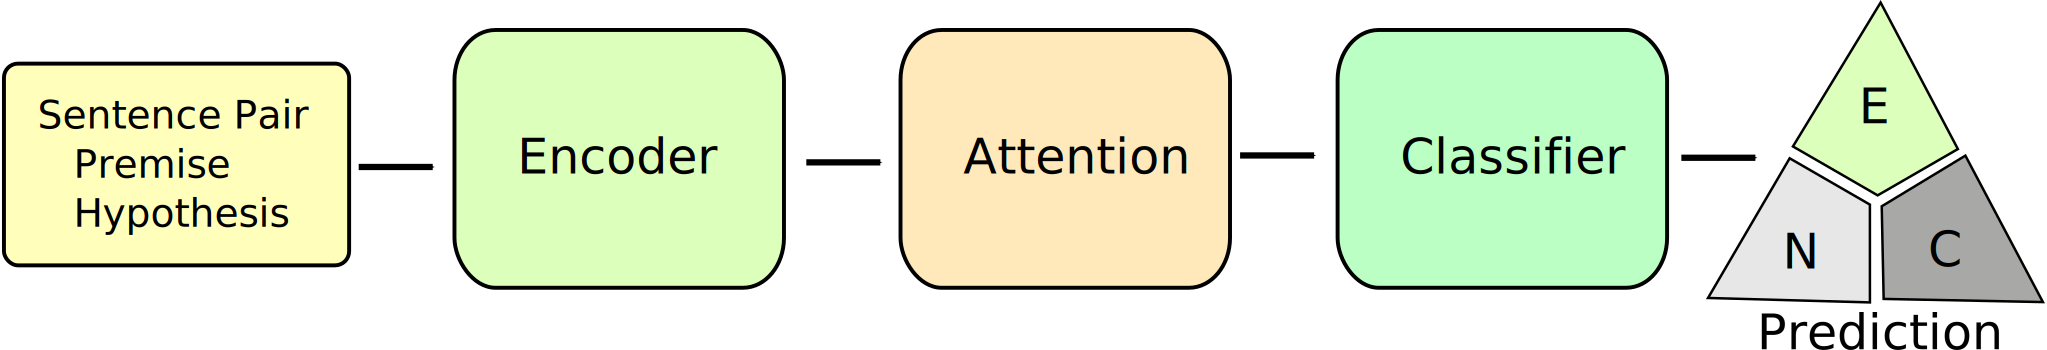
\includegraphics[width=1.0\linewidth]{pipeline}
 \caption{Language Inference Model Pipeline.}
\label{fig:projTransition}
\vspace{-5mm}
\end{figure}


In this work, we introduce a visualization system that through a tight yet flexible integration between visual analytic elements and the underlying model, allow a user to interrogate the model by perturbing the input, the internal state, as well as prediction while observing changes in other parts of the pipeline.
We use natural language inference task~\cite{BowmanAngeliPotts2015} as an example to illustrate how this system help natural language processing (NLP) researchers quickly identify the potential limitation of an NLP model, probe the inner states of the model for interpreting key mechanism such as attention, and ultimately come up with hypothesis on why the model fails.

% ######## Why use perturbation ###########
% Iterate the model design and debug the system hinged on the ability to quickly
% identify the errors made by a model.
%
% Perturbe the input is what NLP researchers have subconsciously been doing to study and test a model.
%
% Interpret/probe the relationship between attention and the prediction result


The key contributions of the proposed works is summarized as the following:
\begin{itemize}
    \item Identify the mistakes made by the model through perturbation of input sentences and visual summarization of the predictions;

    \item Enhance the visual representation of attention by overlaying sentence linguistic structure to allow grammar guided simplification;

    \item Enable the interrogation of the relationship between input sentences, attention, and the prediction by interactively exploring how the change in one of these elements affect other parts of the model.

\end{itemize}

% NLP application using attention
% \begin{itemize}
%     \item Neural translation
%     \item Text summarization
%     \item Text entailment
%     \item Text comprehension (question answering)
% \end{itemize
%
%
% Attention type:
% \begin{itemize}
%     \item soft vs. hard
%     \item local vs. global
%     \item hierarchical
%     \item attention over attention
%     \item gated
% \end{itemize}
